\section{TCTP Impedance Studies}

As part of the ongoing collimation upgrade in the LHC, several advances in the LHC design have been proposed. These are as follows:

\begin{enumerate}
\item{For the reasons given in Sec.~\ref{sec:phase-2-col-mat}, the jaw material of the collimators, specifically the secondary collimators is under review in an effort to reduce the beam impedance, improve cleaning efficiency and continue the present robustness and excellent performance of the LHC collimation system.}
\item{The inclusion of on collimator BPMs. This is due to the present method of alignment of the collimators relying on investigating the beam loss patterns in the LHC as a function of collimator aperture being a very time intensive procedure due to the inherentl slow natyure of beam loss. The use of on collimator BPMs allows a near instantaneous feedback on the position of the beam relative to the collimator jaw thus greatly increasing collimator setup time[cite setup paper gianluca/on collimator BPM paper]}
\item{A new RF system (Shown in Fig.~\ref{fig:phase-2-rf-system}) to reduce the side effects of the sliding RF contacts used in the phase 1 collimators.}
\end{enumerate}

As part of the upgrade, a series of TCTP collimators shall be installed in the LHC in replacement of a number of tertiary collimators (TCTs). In total, 8 TCTP and 1 TCSG will be added to the LHC. These collimators are in part intended to act as a test for two of these upgrades, the use of on collimator BPMs and the new RF system[cite collimators with onboard BPMs]. As part of the ongoing effort to limit increases to the LHC machine impedance (shown in Tab.~\ref{tab:lhc-impedance-budget}) and due to continuing concerns about beam-induced heating [cite cham/evian 2012], all new devices to be placed in the LHC must be examined for their effect on the beam and as a possibly luminuousity limiter in the LHC. Due to the large number of phase 2 secondary collimators that are planned to be put in the LHC (30 additional secondary collimators to be installed during long shutdown 2[cite eucard report]) it is vital that the new collimator design, especially the new RF system is verified for it's efficacy as an impedance reduction technique.  


\begin{table}
\caption{The impedance budgets (both transverse and longitudinal) for LHC. Taken from the LHC Design Report[cite LHC design report 2003-2004]}
\begin{center}
\begin{tabular}{c | c | c}
Beam Operation & Longitudinal $\Im{}m ( Z_{\parallel}/n )$ $( \Omega )$ & Longitudinal $\Im{}m ( Z_{\perp} )$ $( \Omega /m )$\\ \hline
Total Broadband at injection (450GeV) & 0.07 & 1.34 \\ \hline
Total Broadband at collisions with squeezed optics (7TeV) & 0.076 & 2.67 \\ \hline
\end{tabular}
\end{center}
\label{tab:lhc-impedance-budget}
\end{table}


\subsection{TCTP Collimator - Design and Geometry}



\begin{figure}
\subfigure[]{
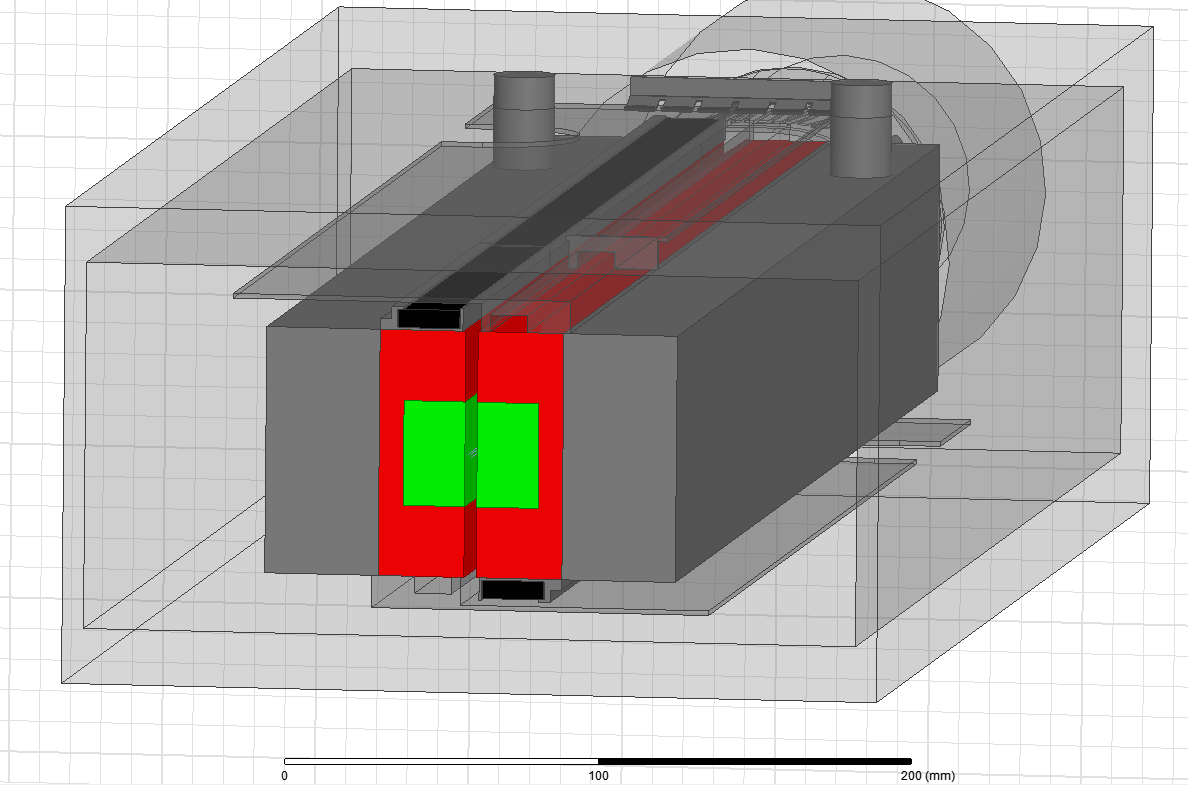
\includegraphics[width=0.45\textwidth]{LHC_Collimation_Upgrades/figures/ferrite_circuit.png}
\label{fig:cross-sec-ferr}
}
\subfigure[]{
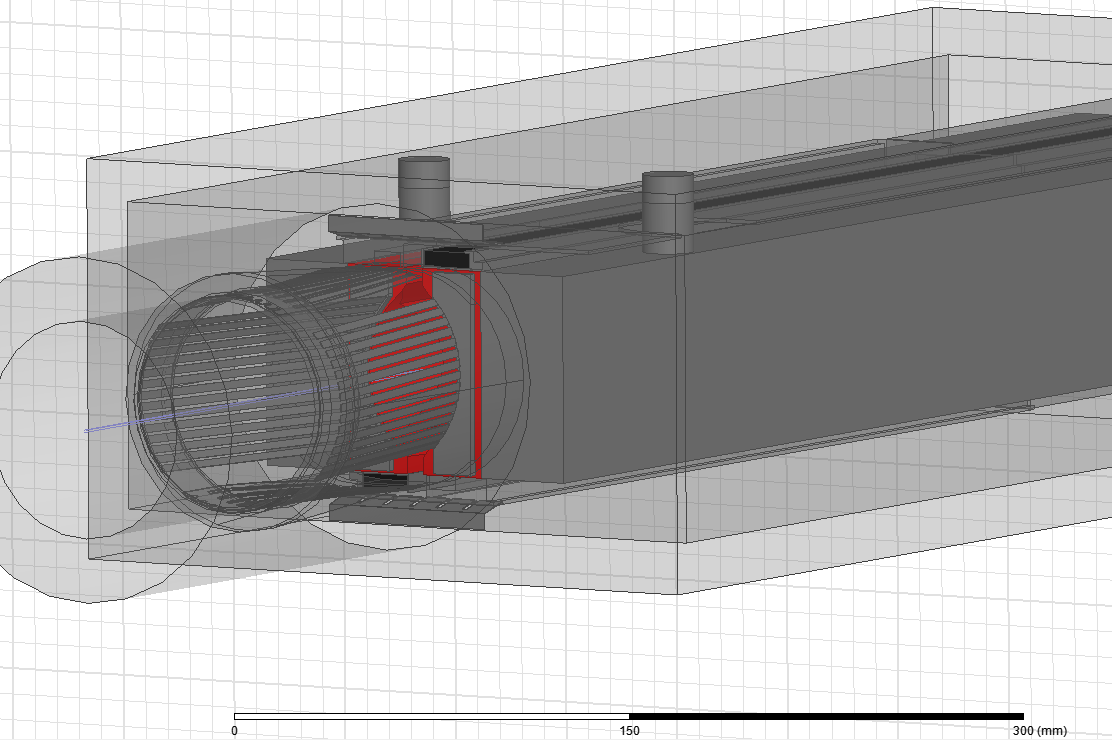
\includegraphics[width=0.45\textwidth]{LHC_Collimation_Upgrades/figures/rf-fingers.png}
\label{fig:cross-sec-rf-fingers}
}
\label{fig:tctp-figure}
\caption{The TCTP collimator has a number of important impedance reduction techniques present in its design. The RF system, \ref{fig:cross-sec-ferr}, replaces the sliding RF contacts of the phase 1 design, using ferrite tiles (shown in black) to reduce the resonant Q of the structure. The longitudinal RF fingers, shown in \ref{fig:cross-sec-rf-fingers}, provide a good conducting path for the beam image current in the transition from the beam pipe to the collimator jaw.}
\end{figure}

The TCTP is a tertiary type collimator with a jaw made of tungsten. The principle components of interest from a beam impedance reduction point of view are the longitudinal RF fingers that cover the transition from the beam pipe to the collimator structure, and the RF system utilising ferrite blocks and a screen structure, shown in Fig.~\ref{fig:cross-sec-ferr}.

The RF system is designed to work in the following way, where comparison is given to the phase 1 RF system to clarify the differences and the design choices made. The phase 1 sliding contacts adequately masked the surrounding vacuum cavity from the beam, causing the resonant modes of the structure to be dominated by the geometry of the internal structure of the collimator jaw. Due to the small dimensions this volume the resonant frequencies are thus very high (in the realm of gigahertz) where the beam spectrum is very small and thus the beam-structure interaction is relatively small thus avoiding both impedance driven instabilities due to cavity modes and beam-induced heating. However the sliding contacts are believed to produce a large quantity of dust which is problematic for beam losses.

Conversely, the TCTP RF system removes the sliding contacts to remove the dust problem. This allows the beam to 'see' the entire vacuum tank of the collimator. This increases the characteristic dimensions driving the resonant frequency modes, thus lowering the minimum frequency of the cavity modes. This moves the frequency of the cavity modes into an area over the beam power spectrum where the spectrum is comparable to the DC beam current in the machine. To counteract this the Q of the cavity modes is reduced by the placement of ferrite tiles in the device to act as a damping material. This strongly reduces the peak height of the impedances thus reducing their effect on both instability and beam-induced heating.